\chapter{On Multimedia Analysis and Retrieval}
\epiquote{All our knowledge begins with the senses, proceeds to the understanding, and ends with reason.}{Immanuel Kant, 1781}
\label{chapter:theory_multimedia_analysis_and_retrieval}

Multimedia refers to the combination of different content forms for the purpose of transport and perception. Over the centuries, countless content forms have been conceived by mankind, natural language being one of the earliest examples. With the invention of the modern computer, more and more of these content forms were transferred to the digital world. Today, multimedia data is ubiquitous and used in different forms in every area of our socioeconomic lives. Statista.com estimates, that the amount of data created, captured, copied, and consumed in 2025 will exceed \SI{181}{\zetta\byte} from an estimated \SI{2}{\zetta\byte} in 2010\footnote{Source: Statista.com, ``Volume of data/information created, captured, copied, and consumed worldwide from 2010 to 2025'', February 2022.}. To a large extent, that data is multimedia data that is being created, stored, analysed and shared for various purposes.

A key development in this regard was the widespread adoption of the smartphone in the early 2000s, which enabled almost every person on this planet to not only consume but also produce multimedia content turning them effectively into prosumers \cite{Ritzer:2010Production,Ritzer2012:Coming}. Fuelled by this technological progress, the past decades have seen a staggering development in both \emph{volume} and \emph{variety} of multimedia data found on the Internet and in commercial and private data collections.

This extreme growth as well as the increasing \emph{velocity} at which data is being produced, poses an enormous challenge for information processing. Therefore, researchers have tried to tackle the questions surrounding the efficient and effective management, analysis and retrieval of multimedia data at a large scale for many decades now, with first attempts reaching back to the early 1970s.

\section{Multimedia Data and Multimedia Collections}
\label{section:multmedia_data}

The term \emph{multimedia} refers to a combination of one or many different \emph{content formats} or \emph{media types}, such as but not limited to observable aural or visual information. We distinguish between these content formats based on the representation we use when working and interacting with them. Raw sound, for example, is formed by air pressure waves that are registered by our ears. In contrast, visual information involves electromagnetic waves captured by our eyes. In both cases, the brain interprets the underlying processes, thus forming the human perception of the phenomenon and the meaning it carries.

Traditionally, we often think of media as information that can somehow be directly observed by our senses. However, since a medium is merely a means to store and transport information, it may also include less apparent and sometimes even digitally native examples such as data streams stemming from sensors, which require specialised hard- and software to allow for observation.

Even though the various types of media may exhibit very different characteristics in their original representation, we find some commonalities that are crucial for formalising the problem of processing and analysing their digital (data) representation (see Examples \ref{example:representation_visual_information} and \ref{example:representation_audio_information}) in information processing systems -- which is our main interest for the purpose of this Thesis.

\begin{description}
    \item[Relationship with Time] At a high level, we can roughly classify all the different media types based on their relationship with time. \emph{Static} media types (e.g., an image) do not exhibit a temporal development, whereas the information in \emph{dynamic} media types (e.g., an audio signal) depends on the time point that is being examined \cite{Blanken:2007multimedia}.

    \item[Unstructured Data] The digital representation of any media type is usually highly unstructured in that there is no connection between the raw data and the higher-level meaning it carries. For example, there is no way to deduce the motives visible in an image just by examining the raw image data. Therefore, information processing systems rely on \emph{derivative representations} of the original data, gained through pre-processing and data analysis.
    
    \item[Semantic Gap] The derivative representations of the original data usually describe specific aspects thereof, and conversion to/from such representations is therefore often accompanied by a loss of information. This is a problem often referred to as the \emph{semantic gap} \cite{Blanken:2007multimedia, Rossetto:2018Multi}.
\end{description}

\begin{example}[label=example:representation_visual_information]{Digital Representation of Visual Information}{}
    \begin{wrapfigure}{L}{0.45\textwidth}
        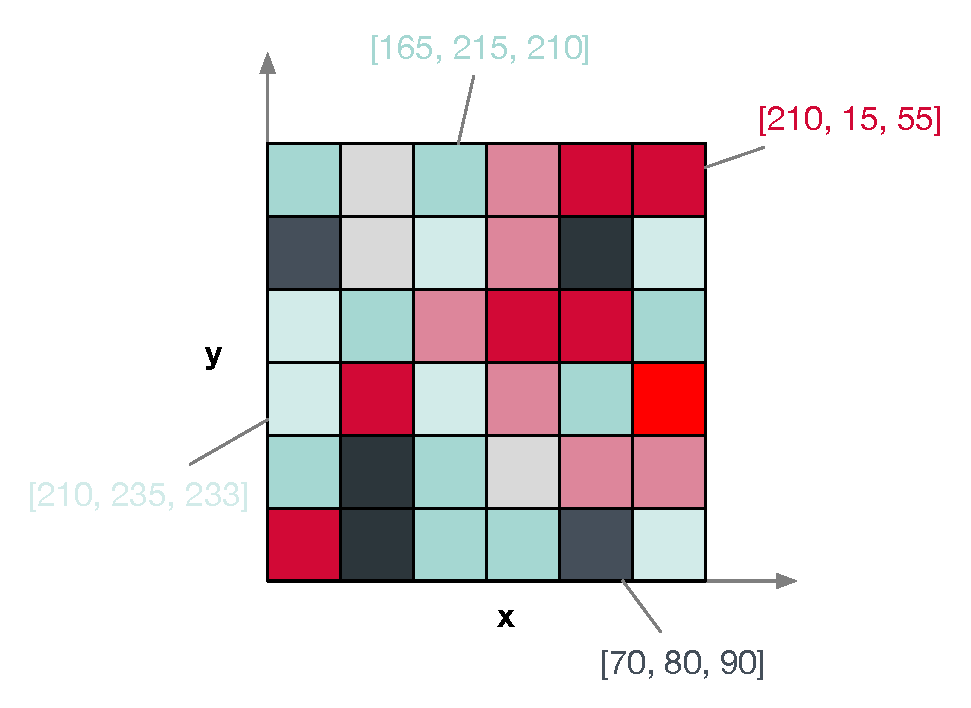
\includegraphics[width=0.45\textwidth]{figures/example-visual-signal.eps}
    \end{wrapfigure}
    The visual information in a flat image is stored as a two-dimensional array of \emph{pixels}. The information in every pixel is typically formed by a sensor, in an array of sensors, that captures the electromagnetic signal. Each pixel holds colour values, usually one per colour channel. For example, with the RGB colour model, every pixel holds three values, one for the red, green and blue channel. The number of pixels per dimension determines the \emph{resolution} of the image. Typically, we use a fixed number of bits per colour -- the \emph{colour depth} -- which determines the number colours that can be distinguished.

    If we take, for example, a coloured image of $1000 \times 1000$ pixels, we must encode \num{3e6} individual colour values. Using \SI{8}{\bit} per colour, we end up storing \SI{24e6}{\bit}, which amounts to \SI{3}{\mega\byte} worth of uncompressed image data. Images coming from modern cameras, exhibit resolutions much higher than that.
\end{example}

\begin{example}[label=example:representation_audio_information]{Digital Representation of Aural Information}{}
    \begin{wrapfigure}{R}{0.45\textwidth}
        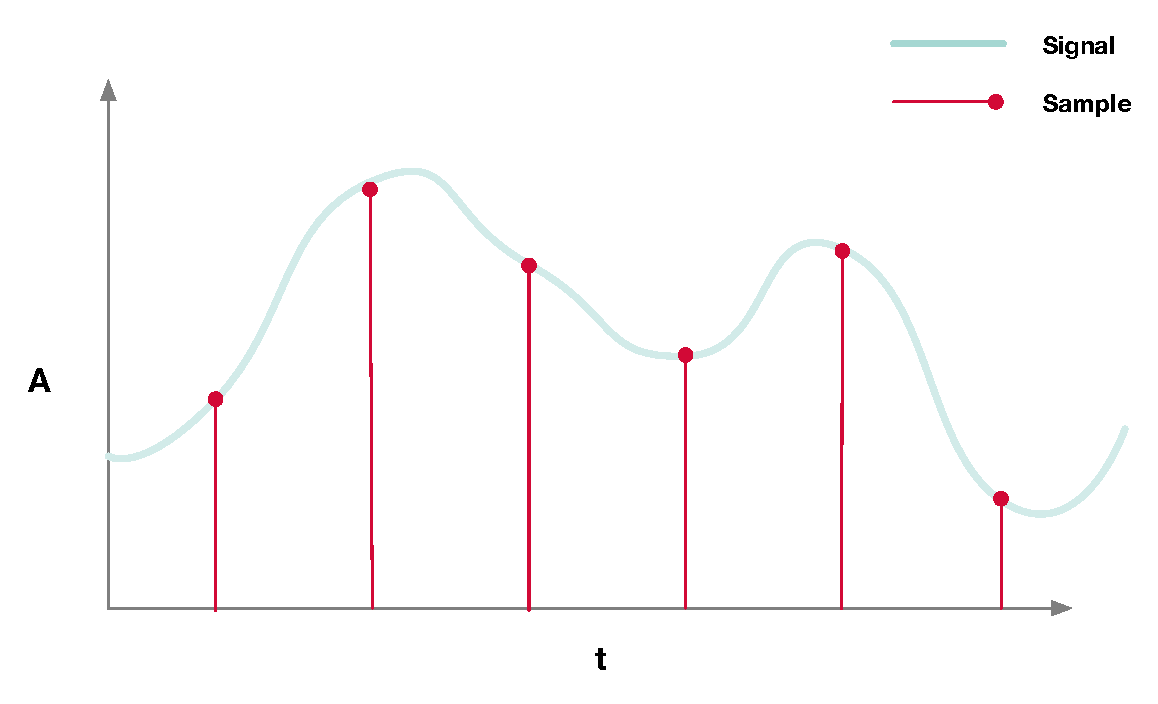
\includegraphics[width=0.45\textwidth]{figures/example-audio-signal.eps}
    \end{wrapfigure}
    The air pressure waves that form sound can be recorded and translated to an electrical signal by microphones. When digitising this information, the temporal development of this signal amplitude is \emph{sampled} at a fixed rate. Each sample point consists of a value that quantises the amplitude's energy at a given point in time to a number on a given range. An audio stream is then a sequence of these values. The quality of the process is determined by the \emph{sample rate}, i.e., the number of samples per time unit, and the \emph{bit depth}, which determines quantisation of the amplitude power.

    If we take a \SI{1}{\second} audio snippet, sampled at \SI{44}{\kilo\hertz}, we end up storing \num{44000} sample points. Using a bit depth of \SI{16}{bit} per sample, this amounts to \SI{704000}{\bit} or \SI{88}{\kilo\byte} of uncompressed audio data. In modern audio systems, we typically record multiple audio channels independently, leading to even more data.
\end{example}

\subsection{A Data Model for (Multi-)Media Collections}
\label{section:media_data_model}
In \Cref{chapter:theory_databases}, we have introduced the notion of a data model and its importance for working with any type of data. Despite being agnostic to the concrete conceptual data model in principle, the work presented in this Thesis still relies on a formal understanding of media data that enables organisation and management thereof. Due to its tight integration into the \emph{vitrivr} project \cite{Rossetto:2016Vitrivr,Gasser:2019Multimodal,Heller:2020Multi}, there is a particular model that we would like to introduce. Under this data model -- which is illustrated in \Cref{figure:erm_mediadata_vitrivr} -- a (multi-)media \emph{collection} consists of multiple (typically a large number of) \emph{media object}s. The media object describes the data at the level of individual documents -- e.g., a video or image file -- and comprises basic attributes such its identifier, its media type, or its path. The path forms the link to the raw media data in the file system, which we assume to be the most suited form of storage for this type of information. That raw data must always be available for processing and presentation.

To account for the temporal development found in dynamic media types, \emph{vitrivr}'s data model has a notion of a \emph{media segment}, which represents a clearly defined temporal slice of the object and stands in a one-to-many relationship with it. However, the model does not make any assumption as to how segments are formed. For static media types, such as images, there is a trivial one-to-one relationship between an object and a segment. For more complex types of media, such as audio or video, media segmentation is a dedicated area of research \cite{Koprinska:2001temporal} and can be approached in many different ways, e.g., at a fixed rate, based on changes in the content \cite{Foote:2000Automatic,Tsai:2016video} or using self-adaptive deep neural networks~\cite{Souvcek:2019transnet}. Obviously, different strategies for segmentation yield different degrees of summarization of information over time. In addition, the proposed distinction also allows for application specific media types and segmentation strategies, such as image sequences -- which were introduced for \acrshort{lsc} 2020 \cite{Heller:2020Interactive} and group images per day for the purpose of lifelog analysis.

To model the different derivative representations that are used to describe a media object and its segments, the model foresees \emph{features}, which again stand in a one-to-many relationship with the segments. That is, every segment can have an arbitrary number of such features that describe different aspects of its content. In practice, different types of features are obtained and stored in dedicated entities. Additionally, \emph{descriptive metadata} allows for a description of the media both at the document and segment level by means of simple key-value pairs that can contain technical metadata, descriptions, labels, or other types of structured information.

\begin{figure}[bt]
    \centering
    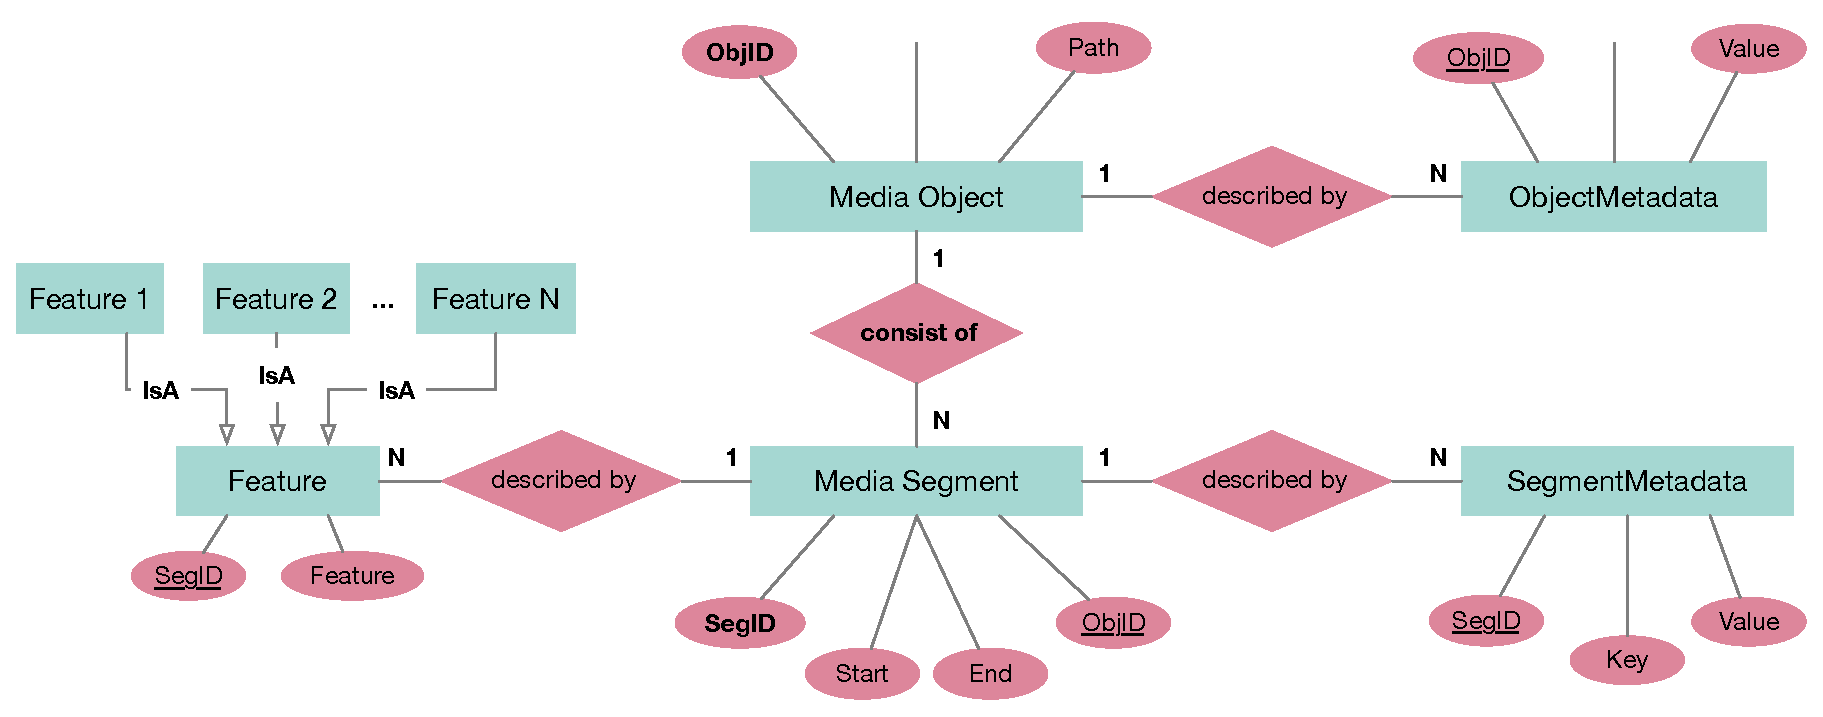
\includegraphics[width=\textwidth]{figures/erm-media-data-vitrivr}
    \caption{An extended \acrshort{erm} of the multimedia data model used in the \emph{vitrivr} project. The model centres around the notion of media objects and media segments which are described by metadata and features.}
    \label{figure:erm_mediadata_vitrivr}
\end{figure}

In this Thesis, we consider a slightly altered version of the aforementioned data model, which is more in line with \cite{Blanken:2007multimedia} and is illustrated in \Cref{figure:erm_mediadata}. This model also considers media objects to be an abstraction of individual files. However, this model foregoes the indirection introduced by the media segment and treats \emph{features}, \emph{annotations} and \emph{descriptions} as different types of a more general \emph{metadata} type that describes the media object directly. To model the temporal aspect in dynamic media types, the metadata itself exhibits information about the part of the object that is being described, denoted by an optional \emph{start} and an \emph{end} marker. In practice, this could be a frame number or a timestamp.

While the difference between the two models may seem marginal, we argue, that the latter offers several advantages over the former: Firstly, it eliminates a level of indirection introduced by the media segment and thus simplifies handling of static media types, which are simply described by different types of metadata that lack a start and end marker. Secondly, it does not assume segmentation to be statically defined and instead makes this a property of the metadata itself. This is reasonable, because the optimal segmentation strategy may depend on a particular feature, especially when multiple media types are involved, e.g., aural and visual information in a video. And finally, the model could be extended to also support spatial information as a basis for segmentation, e.g., in images, which would enable description of spatio-temporal aspects of any media type. However, such ideas are beyond the scope of this Thesis. 

We will use the proposed conceptual data model from \Cref{figure:erm_mediadata} throughout this Thesis and whenever we refer to terms like collection, media object, feature, or descriptive metadata, we refer to the concepts introduced in this model.

\begin{figure}[bt]
    \centering
    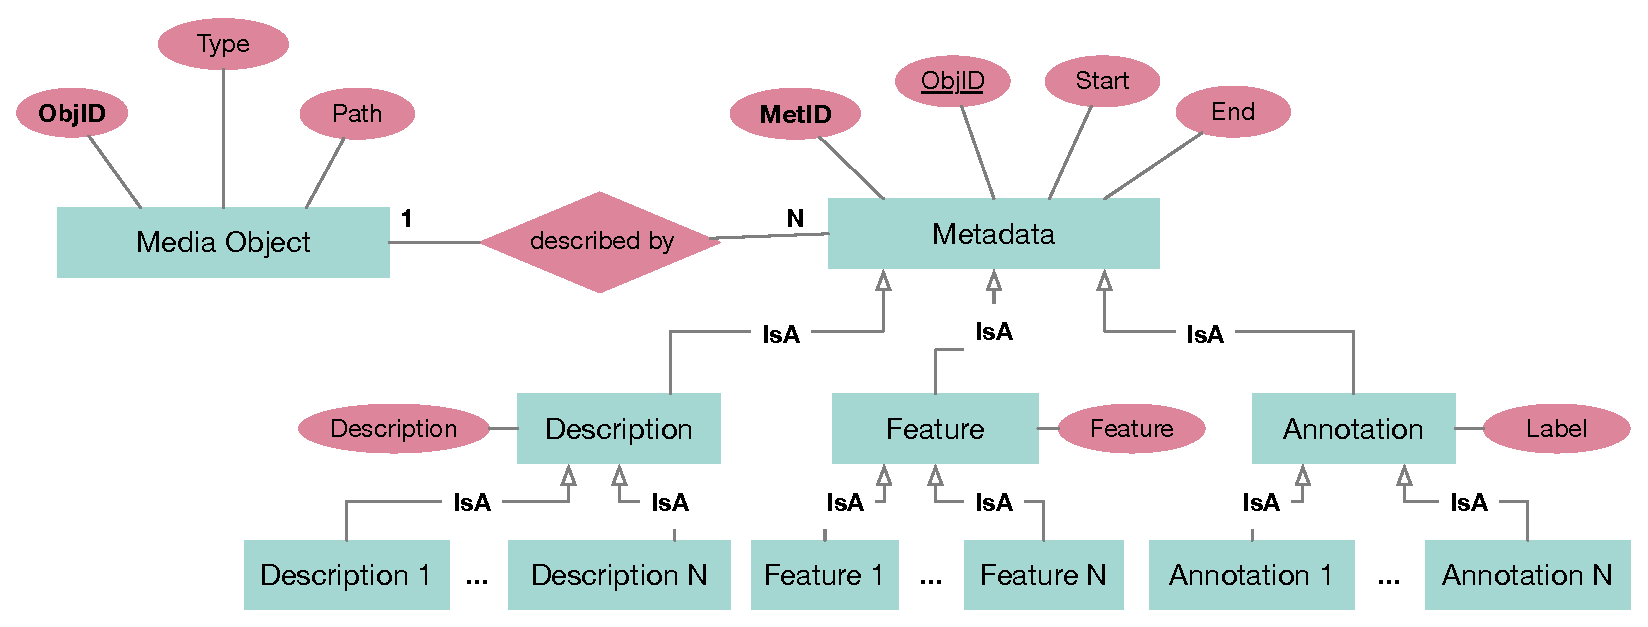
\includegraphics[width=\textwidth]{figures/erm-media-data}
    \caption{An extended \acrshort{erm} of the multimedia data model used for the purpose of this Thesis. It has been derived from \emph{vitrivr}'s data model and foregoes the explicit segment entity.}
    \label{figure:erm_mediadata}
\end{figure}

\subsection{Descriptive Metadata}
Descriptive metadata in the sense of the proposed data model consists of textual descriptions (e.g, title, summary), technical information (e.g., duration, location, frame rate) and annotations (e.g., category labels). Such information has always played an important role in multimedia retrieval and analysis, because it provides (indirect) access to the media's content and can be leveraged in a structured way, e.g., in database queries or for data organisation.

Over the years, many different metadata standards have emerged. ID3\footnote{See https://id3.org/} tags, for example, allow for organisation of large music libraries and classification of songs based on information about artists or albums. Similarly, the Dublin Core Metadata Element Set (DCMES or just Dublin Core)\footnote{See https://www.dublincore.org/} comprises 15 basic properties that can be used to describe any type of media, e.g., videos or images. And last but not least, EXIF\footnote{See https://www.loc.gov/preservation/digital/formats/fdd/fdd000146.shtml/} can be used to describe images and also includes technical metadata, such as the camera model, the exposure time or the f-number. These well-established standards are complemented by a plethora of domain specific standardised and non-standardised metadata frameworks.

However, while useful and important for the problem of analysis and retrieval, this type of metadata comes with important disadvantages. Firstly, and notwithstanding recent developments in machine learning, e.g., in image captioning \cite{Hossain:2019Comprehensive}, such information is traditionally assigned manually in a laborious and time-consuming annotation process. This process is barely able to keep up with the ever-increasing velocity at which new content is created. Secondly, descriptions and labels -- especially if not standardised -- are often subjective due to language, expertise, and personal experience and may therefore differ depending on the person assigning them. This is closely related to the problem of the perceptive and pragmatic gap \cite{Rossetto:2018Multi} and highly relevant for any search process. And finally, it is often challenging to describe the content of media in a textual manner, especially if temporal development is involved.

Regardless of these challenges, however, experience shows that annotations -- be they assigned manually or automatically -- play an important role, especially when it comes to information retrieval. A contributing factor here is that of query formulation, which is very low-effort and familiar for textual input and becomes more challenging for other types of queries.

\subsection{Features}
Simply put, a \emph{feature} is a mathematical object that describes ``derived characteristics''~\cite{Blanken:2007multimedia} of a media object or a part thereof. Therefore, they are sometimes also referred to as \emph{descriptors}. A formal definition is given in \Cref{definition:feature}.

\begin{definition}[label=definition:feature]{Definition of a Feature in Multimedia Analysis}{}
    Let $\symmediacol = \lbrace o_1, o_2, \ldots, o_N \rbrace$ be a collection of media objects $o$ (i.e., files). A \emph{feature} $f_{i,\texttt{start},\texttt{end}} \in \symfeatures$ describes a temporal interval $[ \texttt{start}, \texttt{end} ]$ with $\texttt{start},\texttt{end} \in \symnatural_0, \texttt{start} \leq \texttt{end}$ of the media object $o_i \in \mathcal{C}$ under the feature transformation $\symfeaturetransform$, with 

    \begin{equation}
        \label{eq:feature_transformation}
        \symfeaturetransform \colon \mathcal{C} \times \symnatural_0 \times \symnatural_0 \longrightarrow \mathcal{F}
    \end{equation}

    We call $\symmediacol$ the media object domain and $\symfeatures$ the feature domain. The structure of  $\symfeatures$ is fully determined by $\symfeaturetransform$.
\end{definition}

Features play a central role in many different domains, ranging from mere (multi-)media analysis to retrieval. \cite{Blanken:2007multimedia} distinguishes between low-level and high-level features, which is a qualitative assessment of how far removed the derived characteristic of a particular feature is from a concept that has a semantic meaning to a human user. For example, a histogram of the colours found in an image would be considered a low-level feature, whereas a feature capturing salient key points or even objects in the same image would be classified as high-level. In practice, high-level features are often derived from low-level features, and again these conversions are subject to the semantic gap.

The process of generating features from media objects is called \emph{feature extraction} \cite{Blanken:2007multimedia} and there is an entire corpus of research that deals with the engineering of features that describe the relevant aspects of a given media type's content, with first attempts in computer vision and image understanding dating back to the early 1960s. Various surveys, such as \cite{McKinney:2003Features,Ding:2012ASurvey,Salau:2019Feature}, cover the topic of feature extraction and we simply name and describe a few selected examples to provide an (unrepresentative) overview. Obviously, every type of media has its own analysis techniques that can be used to generate features.

For images, one can roughly distinguish between low-level colour, texture, and shape features \cite{Salau:2019Feature}, as well as higher-level local keypoint-based features. An example of a colour feature could be a simple colour histogram or a statistical moment that captures colour distribution, e.g., the average colour in a defined area of the image. Prominent examples for keypoint detection features include algorithms such as \acrfull{sift}~\cite{Lowe:1999object}, \acrfull{surf}~\cite{Bay:2006surf} or \acrfull{hog}~\cite{Dalal:2005Histograms}. All these features are employed in many different applications ranging from retrieval and similarity search to the detection of higher-level concepts, such as, objects or faces \cite{Deniz:2011Face, Farooq:2016Object}.

Similarly, there is a wide range of features applied in audio analysis and retrieval. \glsentryfirstplural{mfcc} -- a representation of a short-term power spectrum on the perceptual \emph{mel scale} -- play an important role in speaker recognition, sound and music classification as well as audio segmentation \cite{Kim:2010Comparison}. They were shown to outperform audio descriptors outlined in the MPEG-7 standard~\cite{Quackenbush:2001Overview}, which is a collection of standardised feature descriptors for images, audio, and video. Other types of features include \acrfull{pcp} for music retrieval and classification~\cite{Lee:2006Automatic,Demirel:2019Automatic} or features based on rhythm, timbre, or speed. 

So far, we have mostly considered features that were engineered through the careful application of signal processing and/or statistical analysis of the raw media data. However, advances in machine learning and deep neural network architectures have enabled the feature extraction process to be automated to some extent, leading to a shift from  engineered to learned features \cite{Hamel:2010Learning,Gordo:2016Deep}. There is also research that deals with the comparison of the two paradigms in multimedia retrieval and analysis \cite{Budnik:2017learned} as well as other domains, such as chemical structure analysis \cite{Gallegos:2021importance}. Preliminary results show, that while learned features often outperform the engineered ones, best results are attained by a combination of the two.

Given the cornucopia of features and feature extraction techniques to choose from, there are two important aspects that ought to be considered with respect to data modelling and data management: Firstly, the resulting features often exhibit a comparatively simple mathematical structure, despite the vast range of feature extraction techniques. We will show in \Cref{section:multimedia_retrieval} that in multimedia retrieval, one often deals with vectors in a high-dimensional, real-valued vector space \cite{Zezula:2006Similarity}. Secondly, when considering a complex enough use case, no single feature can satisfy all the different types of applications because, as we have pointed out, a specific feature usually focuses on a specific aspect of the content. Consequently, a combination often yields the best results \cite{Deselaers:2008Features}.

Both aspects have important implications for the requirements for a multimedia data management and processing system, especially, if such a system should be able support different use cases that are not necessarily known in advance \cite{Smeulders:2000Content}. We would also like to point out, that both data models introduced in \Cref{section:media_data_model} are flexible enough to handle these two aspects.

\section{Multimedia Retrieval}
\label{section:multimedia_retrieval}

\emph{Multimedia retrieval} deals with algorithms, methods and systems that allow for content-based search and obtaining items of interest from large (multi-)media collections based on user-defined queries. In addition to text-based search, such queries may also involve new modes of query formulation such as \emph{Query-by-Example} \cite{Kelly:1995Query}, \emph{Query-by-Sketch} \cite{Cao:2010mind}, \emph{Query-by-Humming} \cite{Ghias:1995query}, or \emph{Query-by-Sculpting} \cite{Boerlin:20203d}. Many different research domains for the different types of media have emerged over the years, including but not limited to content-based image retrieval \cite{Dharani:2013Survey}, audio retrieval \cite{Lu:2001Indexing}, video retrieval \cite{Hu:2011Survey}, 3D model retrieval \cite{Yang:2007Content} and various subdomains \cite{Murthy:2018Content}.

Formally, the multimedia retrieval problem can be characterised as finding all media objects $o \in \symmediacol$ that may be relevant to a given \emph{information need} expressed by a user as query $q$. This is achieved by obtaining some form of \emph{(dis-)similarity}\footnote{Depending on the context, the likeness of an object to a query may be directly (similarity) or inversely (dissimilarity) proportional to the obtained score.} between $q$ and $o$ and ranking results based on it, which is why the method is also referred to as \emph{similarity search}. In contrast to Boolean search with its strict match/miss-semantic, the results produced by similarity search are non-binary in the sense that an object $o$ may match a query $q$ only to a certain degree but still be considered part of the resultset.

Since a direct comparison of a media object to a query is often not feasible -- for reasons described in \Cref{section:multmedia_data} -- features are used as a proxy instead. This is a manifestation of the idea that derivative representations are considered in lieu of the actual object, leading to the formal \Cref{definition:similarity_search} of similarity search.

\begin{definition}[label=definition:similarity_search]{Similarity Search}{}
    Let $\symmediacol = \lbrace o_1, o_2, \ldots, o_N \rbrace$ be a media collection of media objects $o$ and let further $\symfeatures$ be a feature domain of $\symmediacol$ under the feature transformation $\symfeaturetransform$. Furthermore, we assume a query $q \in \symfeatures$ and the existence of an inverse $\symfeaturetransform^{'}$ with $\symfeaturetransform^{'}(f) = o$ \footnote{While this may seem like a preposterous assumption at first, this is a given since we explicitly store the relationship between $o$ and $f$, according to the data model in \Cref{section:multmedia_data}.}.

    Similarity search then is the optimisation problem of finding the object $o \in \symmediacol$ that given a query $q$ and a similarity function $\symsim \colon \symfeatures \times \symfeatures \rightarrow [0, 1]$ maximises the following expression.

    \begin{equation}
       o_r =  \symfeaturetransform^{'} (\argmax_{f \in \symfeatures} \symsim(f,q))
    \end{equation}
 
    We call the resulting item $o_r$ most similar with respect to $q$, which is indicated by the similarity score $\symsim(f,q)$. In practice, we may be interested in the top $k$ results rather than just a single item.
\end{definition}

In simple terms, a multimedia retrieval system operates upon features $f \in \symfeatures$ derived from the original media objects by means of a feature transformation. This transformation is applied twice: Once when indexing a media object in the collection -- often a step that is thought of as taking place offline -- and once when deriving the same feature from the query input provided by the user, leading to $q$. Subsequently, the system generates the similarity measure $\symsim(q,f)$ which quantifies the similarity between $q$ and $f$ from low ($0.0$) to almost identical ($1.0$) and selects the top $k$ entries that maximise this score. The flow of information that results from this approach is illustrated in \Cref{figure:multimedia_retrieval_flow}. 

Oftentimes, the function $\symsim$ may not express similarity but rather dissimilarity between objects, in which case we can simply consider the dual problem. Furthermore, the score may not always be normalised to $[0, 1]$, which makes it difficult to combine scores of multiple features, e.g., in \emph{score-based late fusion} \cite{Depeursinge:2010Fusion,Rossetto:2018Multi}. However, a normalised similarity score can always be derived by applying an additional correspondence function $\symcorr \colon \symreal_{\geq 0} \rightarrow [0, 1]$. Both aspects are of high practical relevance, but they do not alter the basic problem. 

\begin{figure}[tb]
    \centering
    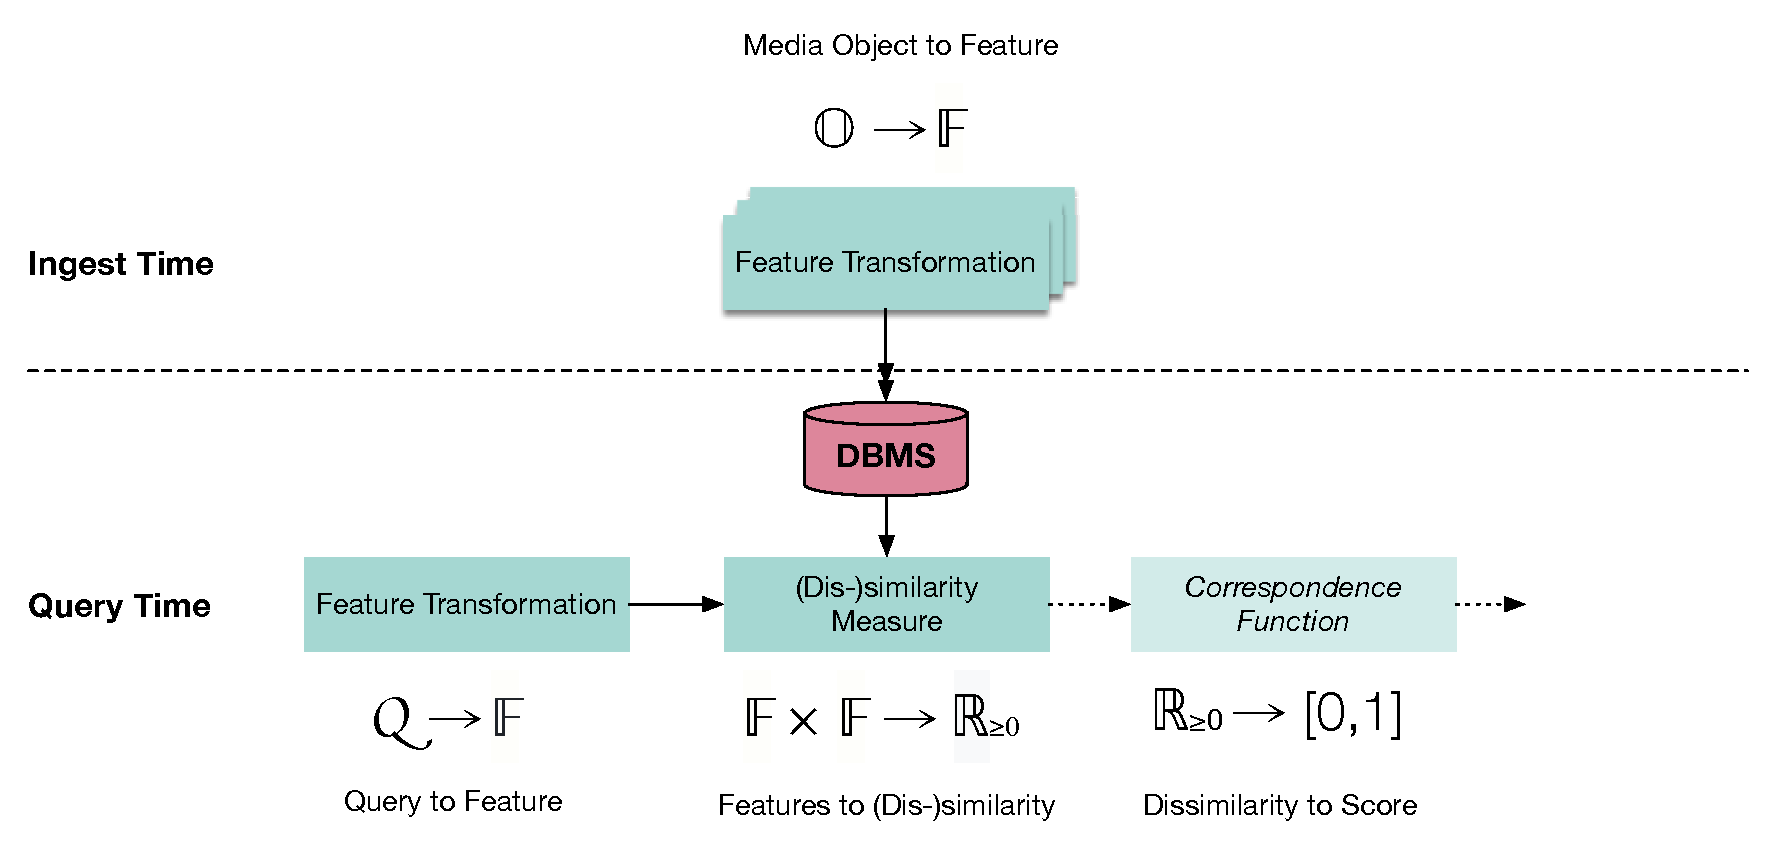
\includegraphics[width=\textwidth]{figures/multimedia-retrieval-pipeline}
    \caption{Flow of information in similarity search at ingest and query time.}
    \label{figure:multimedia_retrieval_flow}
\end{figure}

\subsection{Similarity Search and the Vector Space Model}

The \emph{vector space model} of similarity search \cite{Salton:1975Vector} assumes that the domain of the feature vectors $\symfeatures$ is a subset of a mathematical vector space -- that is, a set whose elements may be added and multiplied by a scalar. In practice, we often consider that vector space to be real-valued and high-dimensional, i.e., $\symfeatures \subset \symreal^{d}$ wherein $d$ is the dimension and an inherent property of the feature and the underlying transformation $\symfeaturetransform$. Consequently, every feature $f \in \symreal^{d}$ is simply a point in that high-dimensional vector space.

Under this premise, we consider the dissimilarity function $\symdist(f,q)$ to be a function that calculates the distance between a feature and a query $f,q \in \symfeatures$, as defined by \Cref{eq:distance_function}. Typically, the farther two vectors lie apart under the distance measure, the more dissimilar they are, which is why we also call this proximity-based search. A list of important distance functions used in similarity search is given in \Cref{table:similarity_measures}. 

\begin{equation}
    \label{eq:distance_function}
    \symdist \colon \symfeatures \times \symfeatures \rightarrow \symreal
\end{equation}

\begin{table}[hb]
    \begin{tabular}{ | c | c | c | c | c | c |}
        \hline
        \textbf{Name} & \textbf{Symbol} &  $\symdist \mathbf{(f,q)}$ & \textbf{Domain} & \textbf{Co-Domain} & \textbf{Metric} \\
        \hline
        \hline 
        Manhattan & $L^1$ & $\sum_{i=1}^{d} | f_i - q_i |$ & $\symreal^d$ & $\symreal$ & metric \\ 
        \hline
        Euclidean & $L^2$ & $\sqrt{\sum_{i=1}^{d} (f_i - q_i)^2}$ & $\symreal^d$ & $\symreal$ & metric \\  
        \hline
        Minkowski & $L^p$ & $\sqrt[p]{\sum_{i=1}^{d} (f_i - q_i)^p}$ & $\symreal^d$ & $\symreal$ & metric if $p \in \symnatural_{\geq 1}$ \\ 
        \hline
        Chi-Square & $\chi^2$ & $\sum_{i=1}^{d} \frac{(f_i - q_i)^2}{f_i + q_i}$ & $\symreal^d$ & $\symreal$ & metric \\ 
        \hline
        Kullback-Leibler & - & $\sum_{i=1}^{d} q_i \log (\frac{q_i}{f_i})$ & $\symreal^d$ & $\symreal$ & non-metric \\ 
        \hline
        Cosine & - & $1 - \frac{\sum_{i=1}^{d} f_{i}q_{i}}{\sqrt{\sum_{i=1}^{d} f_i^2} \sqrt{\sum_{i=1}^{d} q_i^2}}$ & $\symreal^d$ & $[-1, 1]$ & semi-metric \\  
        \hline
        Jaccard & - & $1 - \frac{A \cap B}{A \cup B}$ & $\symfeatures$ & $[0, 1]$ & metric \\
        \hline
        Levenshtein \cite{Levensthtein:1965Binary} & - & - & $\mathbb{S}$ & $\symnatural$ & metric \\
        \hline
        Hamming & - & - &  $\mathbb{S}$ & $\symnatural$ & quasi-metric \\
        \hline
        LCS \cite{Hirschberg:1977Algorithms} & - & - &  $\mathbb{S}$ & $\symnatural$ & non-metric \\
        \hline
    \end{tabular}
    \caption{List of distance functions often used in similarity search.}
    \label{table:similarity_measures}
\end{table}

In broad terms, one can distinguish between \emph{continuous} and \emph{discrete} distance functions \cite{Zezula:2006Similarity}. Continuous functions typically exhibit a very large, potentially infinite co-domain whereas discrete functions map to a limited, often pre-defined set of values. Furthermore, some distance functions induce a topology on the underlying vector space -- often denoted as  \emph{metric space} $(\symfeatures, \symdist)$. We call these \emph{metric distances}, and they satisfy the \emph{non-negativity}, \emph{symmetry}, \emph{identity of indiscernibles}, and \emph{triangle inequality}. 

\begin{align}
  \label{eq:metric}
   \symdist(f,q) &\geq 0                           \tag{non-negativity} \\
   \symdist(f,q) &= \symdist(q,f)                    \tag{symmetry}\\
   \symdist(f,q) &= 0 \Longleftrightarrow f = q    \tag{identity of indiscernibles}\\
   \symdist(f,q) &\leq  \symdist(f,g) +  \symdist(g,q)   \tag{triange inequality}\\
   \forall f,g,q \in \symfeatures \wedge (\symfeatures, \symdist) \nonumber
\end{align}

The constraints imposed on a metric space give rise to mathematical properties that can be exploited for efficient execution of similarity search and specialised indexing techniques \cite{Zezula:2006Similarity}. However, despite their mathematical convenience, some applications involve distances that do not exhibit all the aforementioned properties of a metric, e.g., quasi-metrics (lack symmetry), semi-metrics (lack triangle inequality), meta-metrics (lack identity) \cite{Zezula:2006Similarity}, or even necessitate the use of non-metric functions \cite{Skopal:2011Nonmetric}.

The choice of (dis-)similarity measure mainly depends on the application. All the Minkowski distances (i.e., $L^1$, $L^2$, $L^p$) can be used for any type of real-valued vector and in practice, it often makes little difference which one is employed \cite{Rossetto:2018Multi}. Of all the Minkowski distances, the Euclidean distance ($L^2$) is the most common. The Chi-squared distance is well suited, if the feature vectors represent histograms \cite{Pele:2010Quadratic}. The Hamming and Levenshtein \cite{Levensthtein:1965Binary} distances belong to the class of \emph{edit distances} and can be used to compare strings.

In the following sections, we will explore different variants of the similarity search problem, which are all variants of \Cref{definition:similarity_search} and illustrated in \Cref{fig:sim_search_algorithm} and \Cref{example:similarity_search}.

\subsubsection{\texorpdfstring{\acrfull{nns}}{Nearest Neighbour Search (NNS)}}

\acrshort{nns} is probably one of the most prominent types of queries used in multimedia retrieval and certainly the one employed most often in the context of the \emph{vitrivr} \cite{Rossetto:2016Vitrivr,Gasser:2019Multimodal} stack. Given the query object $q$ and an arbitrary limit $k \in \symnatural$, the task is to find the $k$ features $f \in \symfeatures$ that are closest to $q$ as illustrated in \Cref{fig:knn}. This is also referred to as \acrfull{knn}. Formally, the resultset $R$ is given by \Cref{eq:knn}.

\begin{equation}
    \label{eq:knn}
    \lbrace R \subset \symfeatures \colon \forall f_r \in R, f \in \symfeatures \setminus R, \symdist(q,f_r) \leq \symdist(q,f) \wedge |R| = k \rbrace
\end{equation}

Algorithmically, the distance between all $f \in \symfeatures$ and $q$ must be evaluated exhaustively and the top $k$ results must be retained by ranking and ordering the results, e.g., in a \emph{bound priority queue}. This is sometimes referred to as the \emph{brute-force} approach to \acrshort{nns}. For $\symfeatures \subset \symreal^d$, its runtime complexity is $\mathcal{O}(dN)$ and thus depends linearly on the cardinality $N = |\symfeatures|$ and the dimension $d$. 

A variant of \acrshort{knn} is \acrfull{kfn} wherein instead of the nearest, the farthest neighbours are obtained. This can be useful, for example, to obtain negative examples to train recommender systems \cite{Pagh:2015Approximate}. However, the underlying algorithm remains the same.

\subsubsection{Range Search}

Range search -- or $\epsilon$NN -- is useful for finding objects that lie within a given range, typically expressed by a value $\epsilon \in \symreal$. Given the query object $q$, the task is to find all features $f \in \symfeatures$ that lie within $\epsilon$ of $q$ as illustrated in \Cref{fig:enn}. Formally, the resultset $R$ is given by \Cref{eq:epsilonnn}.

\begin{equation}
    \label{eq:epsilonnn}
    \lbrace R \subset \symfeatures \colon \forall f_r \in R, \symdist(q,f_r) \leq \epsilon \rbrace
\end{equation}

Algorithmically, this search strategy is similar to \acrshort{nns} in that all features must be evaluated exhaustively and in that its complexity for $\symfeatures \subset \symreal^d$ is $\mathcal{O}(dN)$. However, in contrast to \acrshort{nns}, there is no need for intermediate sorting, since the selection is based on a simple numerical comparison to the constant $\epsilon$.

Variants of $\epsilon$NN include instances, where $f$ must be larger than $\epsilon$ or where $f$ must fall into an interval $[ \epsilon_{l}, \epsilon_{u} ]$. However, these variants are equivalent to the base case since only the selection predicate changes.

\subsubsection{\texorpdfstring{\acrfull{rnns}}{Reverse Nearest Neighbour Search (RNNS)}}

In \acrshort{rnns} \cite{Korn:2000Influence} we try to find all $f \in \symfeatures$ that given a limit $k \in \symnatural$ consider the query $q \in \symfeatures$ to be part of their \acrshort{knn} resultset as illustrated in \Cref{fig:rknn}. Formally, the resultset $R$ is given by \Cref{eq:rknn} 

\begin{equation}
    \label{eq:rknn}
    \lbrace R \subset \symfeatures \colon \forall f_r \in R, q \in \texttt{kNN}(f_r) \wedge f \in \symfeatures \setminus R \colon q \in \texttt{kNN}(f)  \rbrace
\end{equation}

Algorithmically, this type of search is more complex than \acrshort{knn} or $\epsilon$NN, because basically, a \acrshort{nns} problem must be solved for every element $f \in \symfeatures$. Therefore, the runtime complexity is $\mathcal{O}(dN^2)$ and scales with the square of $N = |\symfeatures|$. 

\begin{example}[label=example:similarity_search]{Comparing different types of similarity search algorithms}{}
    For this example, we consider $f \in \symfeatures \subset \symreal^2$ to be points of interest (e.g., museums, hotels, parks) on a two-dimensional city map. Furthermore, we consider $q \in \symfeatures$ to be another position on the same map, e.g., given by our current position or a selected point of interest. The different types of similarity queries can now be thought of as follows:

    \begin{description}
        \item[Nearest Neighbour Search] is the equivalent of finding the $k$ points of interest that are closest to $q$ (e.g., the three museums closest to my location).
        \item[Range Search] is the equivalent of finding all points of interest that are within $\epsilon$ distance from  $q$ (e.g., all museums within \SI{3}{km} from my location).
        \item[Reverse Nearest Neighbour Search] is the equivalent of finding all points of interest that consider $q$ to be among their closest points of interest (e.g., finding all hotels that have a specific museum in the set of their three closest sites that must be seen when visiting the city).
    \end{description}
\end{example}

\begin{figure}
    \centering
    \begin{subfigure}[b]{0.25\textwidth}
        \centering
        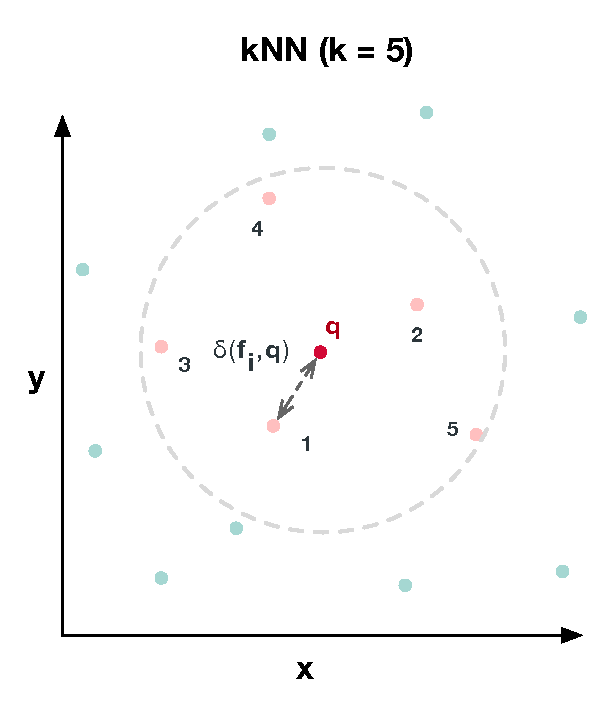
\includegraphics[width=\textwidth]{figures/knn}
        \caption{kNN}
        \label{fig:knn}
    \end{subfigure}
    \hfill
    \begin{subfigure}[b]{0.25\textwidth}
        \centering
        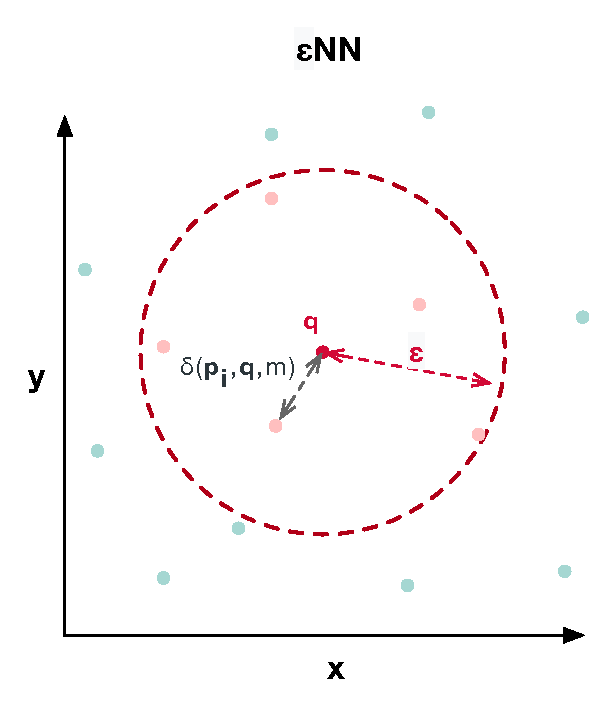
\includegraphics[width=\textwidth]{figures/enn}
        \caption{$\epsilon$NN}
        \label{fig:enn}
    \end{subfigure}
    \hfill
    \begin{subfigure}[b]{0.25\textwidth}
        \centering
        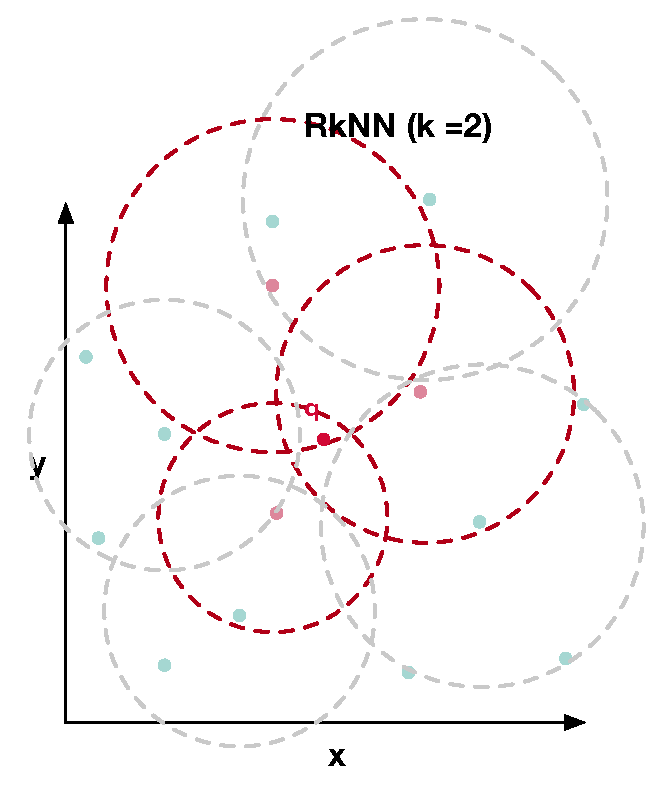
\includegraphics[width=\textwidth]{figures/rknn}
        \caption{RkNN}
        \label{fig:rknn}
    \end{subfigure}
    \caption{Illustration of the different similarity search algorithms in $\symfeatures \subset \symreal^2$ using the Euclidean distance ($L^2$). Matches are highlighted in red.}
    \label{fig:sim_search_algorithm}
\end{figure}

\subsection{\texorpdfstring{\acrshort{nns}}{NNS} and High-Dimensional Index Structures}
\label{section:hd_index_structures}

As we have argued in \Cref{section:multimedia_retrieval}, even the simple \acrshort{nns} problem in $\symreal^d$ exhibits a non-negligible runtime complexity of $\mathcal{O}(dN)$ for a linear brute-force scan -- thus being proportional to the cardinality $N = |\symfeatures|$ and the dimension $d$. Experience from database research shows that linear scans are too slow in terms of time required for query execution if $N$ becomes large enough, especially when interactive query workloads are involved. This necessitates the use of index structures that allow for sub-linear data access.

The dependency on $d$ has a major impact on the execution performance of any search algorithm, due to what is known as the \emph{curse of dimensionality} \cite{Beyer:1999Nearest,Zezula:2006Similarity}. The impact of this ``curse'' is threefold: Firstly, the execution time of a brute-force algorithm is directly proportional to the dimension. With a tendency towards more complex and thus higher-dimensional vectors, there is a negative effect on runtime. Secondly, the distances between a query and the closest and the farthest point tend to become indistuingishable as dimensionality increases \cite{Beyer:1999Nearest}. And finally, research has shown that traditional approaches, e.g., based on partitioning or classical tree structures, degenerate for higher dimensions \cite{Indyk1998:Approximate,Weber:1998Va} with the consequence, that they yield only marginal or no improvement over executing a linear scan. In fact, it was formally proven in \cite{Shaft:2006Theory} that the performance of almost all known index structures at that time deteriorates to that of a linear scan if $d$ becomes large enough.

Nevertheless, the issue of index structures that allow for more efficient \acrshort{nns} was taken on by various researchers and is still an active area of research with results of high practical relevance. At a high-level, indexing algorithms can be classified along three dimensions: Firstly, based on whether they provide any guarantees with respect to the quality of the results, wherein quality is often measured in terms of precision and recall of a result produced by an index as compared to the result produced by a linear scan \cite{Echihabi:2021High}. Since a majority of established techniques sacrifice quality for speed \cite{Siguroardottir:2005Quality}, this is also known as \acrfull{anns}. Secondly, based on their \emph{organisation structure} \cite{Shaft:2006Theory}, e.g., graph and inverted index \cite{Sivic:2003Video} or multi-index \cite{Babenko:2014Inverted}. And finally, by the method that is employed, e.g., \emph{quantisation}, \emph{hashing}, \emph{partitioning}, or \emph{clustering}. An overview of different algorithms is provided in \Cref{table:index_structures}.

\begin{table}
    \begin{tabular}{ | l | c | c | c |}
        \hline
        \textbf{Name} & \textbf{Guarantees} & \textbf{Structure} & \textbf{Method} \\
        \hline
        \hline
        KDB-Tree \cite{Robinson:1981KDB} & exact & tree & space partitioning \\  
        \hline
        $R^{*}$-Tree \cite{Beckmann:1990RTree} & exact & tree & data partitioning \\ 
        \hline
        \acrshort{vaf} \& VA+ \cite{Weber:1998Va,Ferhatosmanoglu:2000Vector} & exact & list & scalar quantisation \\ 
        \hline
        \acrshort{lsh} \cite{Indyk1998:Approximate, Wang:2017ASurvey} & approximate, probabilistic & inverted index & hashing \\ 
        \hline
        \acrshort{pq} \cite{Jegou:2010Product} & approximate & list / inverted index & vector quantisation \\
        \hline 
        \acrshort{cp} \& e\acrshort{cp} \cite{Chierichetti:2007Finding,Gudmundsson:2010Large} & approximate & inverted index & clustering \\ 
        \hline
        NV-tree \cite{Lejsek:2009NVTree} & approximate & tree & scalar quantisation \\ 
        \hline
        NGT \cite{Iwasaki2016:Pruned} & approximate & graph / tree & proximity graph \\ 
        \hline
        MRNG \cite{Lejsek:2009NVTree} & approximate & graph & proximity graph \\ 
        \hline
        HNSW \cite{Malkov:2018Efficient} & approximate & graph & proximity graph \\ 
        \hline
        SPANN \cite{Chen:2021SPANN} & approximate & graph & proximity graph \\ 
        \hline
    \end{tabular}
    \caption{Non-exhaustive list of high-dimensional index structures employed in similarity search and retrieval.}
    \label{table:index_structures}
\end{table}

Early examples of high-dimensional indexes mainly relied on space or data partitioning, i.e., they assigned features to buckets or data files based on some partitioning of either the vector space \cite{Bentley:1975Multidimensional,Robinson:1981KDB,Finkel:1974Quad} or the data \cite{Guttmann:1984RTrees,Beckmann:1990RTree,Ciaccia:1997Mtree}. While these indexes were able to produce exact results, the speed-up they could provide quickly diminished as dimensionality increased due to the aforementioned dimensionality curse \cite{Shaft:2006Theory}, which led to the inception of approximate technique such as \acrshort{lsh} \cite{Indyk1998:Approximate} or \acrshort{pq} \cite{Jegou:2010Product}.

Recent research in high-dimensional indexing focuses on the use of graphs \cite{Shimomura:2021Survey}, for example, proximity \cite{Zhao:2022Approximate} or \acrfull{hnsw} graphs \cite{Malkov:2018Efficient,Chen:2021SPANN}, to facilitate fast \acrshort{anns}. Another focus lies on the ability to execute \acrshort{nns} indexing and search on a GPU \cite{Johnson:2019Billion,Zhao:2020Song} or specialised hardware \cite{Lee:2022Anna}, dynamic indexing, i.e., indexes that allow for online processing of changes to the data \cite{Olafsson:2011Dynamic,Zhao:2022Approximate} and disk-based indexing \cite{Jayaram:2019DiskANN}. In the next few sections, we will highlight a few, selected examples of high-dimensional index structures.

\subsubsection{\texorpdfstring{\acrfull{vaf}}{Vector Approximation File (VAF)}}
\label{section:index_vaf}

VA files were proposed by Weber et al. \cite{Weber:1998Va} to address the problem of the dimensionality curse. The basic idea of a \acrshort{vaf} is the division of the data space into $2^b$ cells, as illustrated in \Cref{fig:vaf}, where $b$ denotes a fixed number of bits. Typically, one chooses a specific number of bits per dimension $b_d$ and uniformly partitions the vector space along each dimension, i.e., $b = b_dd$. A feature's position in the resulting lattice is concatenated into a compact \emph{signature} of size $b$ and the VA file constitutes a list of those signatures. 

\begin{figure}[tb]
\centering
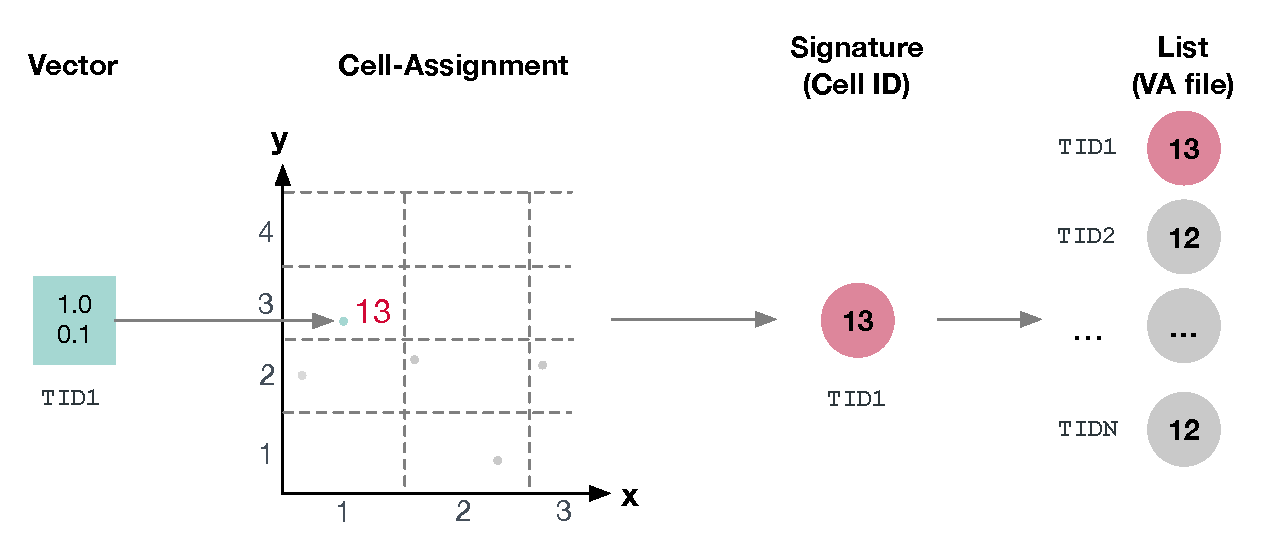
\includegraphics[width=0.95\textwidth]{figures/vaf}
\caption{Simplified illustration of basic \acrshort{vaf} indexing scheme in for $\symfeatures \subset \symreal^2$. A vector is assigned to a cell in an overlay grid, which gives rise to a signature that is stored in a linear list with the vector or its tuple identifier.}
\label{fig:vaf}
\end{figure}

\acrshort{nns} is then realised as a linear scan of the VA file. Speed-up over a brute-force scan of the original vectors is achieved in two ways: Firstly, the signatures are more compact than the original representation ($b$ bits per dimension), i.e., it reduces \acrshort{io} cost through scalar quantisation. Secondly, the signatures can be used to obtain approximate bounds that are computationally less expensive than the actual distance calculation. These bounds can be used to filter out a majority of the points in the file, further reducing \acrshort{io} and CPU costs. Experimental results presented in \cite{Weber:1998Va} demonstrate that more than 90\% of all features can be skipped and thus a distance must only be obtained for the remaining 10\%. However, VA files remain linear in nature and \cite{Echihabi:2021High} determine analytically that for \acrshort{vaf}, a degeneration is still to be expected for high dimensions. Nevertheless, a huge advantage of the \acrshort{vaf} index is, that it does neither sacrifice precision nor recall to obtain speed-up.

The VA+ files described by \cite{Ferhatosmanoglu:2000Vector} are an extension to the \acrshort{vaf} and introduce a few optimisations to the original algorithm, which implicitly assumes independence of the individual dimensions within a feature (which is often not a given). They suggest a prior decorrelation of the individual dimensions by applying a \acrfull{klt}. Furthermore, they propose a non-uniform assignment of bits per dimension, based on data distribution, as opposed to a uniform distribution employed in the original paper. This leads to an independent quantiser per transformed dimension. Results suggest that these adjustments lead to a better estimation of lower and upper bounds, which improves the VA file's filtering capabilities and thus further reduces \acrshort{io} cost.

\subsubsection{\texorpdfstring{\acrfull{lsh}}{Locality Sensitive Hashing (LSH)}}

\acrshort{lsh} refers to a family of algorithms \cite{Echihabi:2021High,Wang:2017ASurvey} that all share the same basic idea of \emph{locality preserving hashing} as first proposed by \cite{Indyk1998:Approximate}. The idea is centred around a hash function $h: \symfeatures \rightarrow B$ that maps any two points $f,q \in \symfeatures$ to a bucket $b \in B$ such that Equations \ref{eq:lsh_1} and \ref{eq:lsh_2} hold, wherein $(\symfeatures, \symdist)$ must constitute a metric space, $P_1, P_2 \in [0, 1], P_1 > P_2$ denote probabilities, $R > 0$ denotes an arbitrary threshold and $c > 1$ denotes an approximation factor.

\begin{eqnarray}
    \symdist (p,q) \leq R \Rightarrow h(f) = h(q) \text{ with a probability of at least } P_1 \label{eq:lsh_1} \\
    \symdist (p,q) \geq cR \Rightarrow h(f) = h(q) \text{ with a probability of at most } P_2 \label{eq:lsh_2}
\end{eqnarray}

In simple terms, a locality preserving hash function has a high probability for collision (i.e., mapping to the same bucket) if two features $f,q \in \symfeatures$ lie close to one another, i.e., $\symdist(q,f) \leq R$, but exhibits a low probability for collision if $\symdist(q,f) \geq cR$. A  feature $f \in \symfeatures$ can then be hashed to a bucket and stored in a hash table with other vectors that lie close to it as illustrated in \Cref{fig:lsh}. 

\begin{figure}[tb]
    \centering
    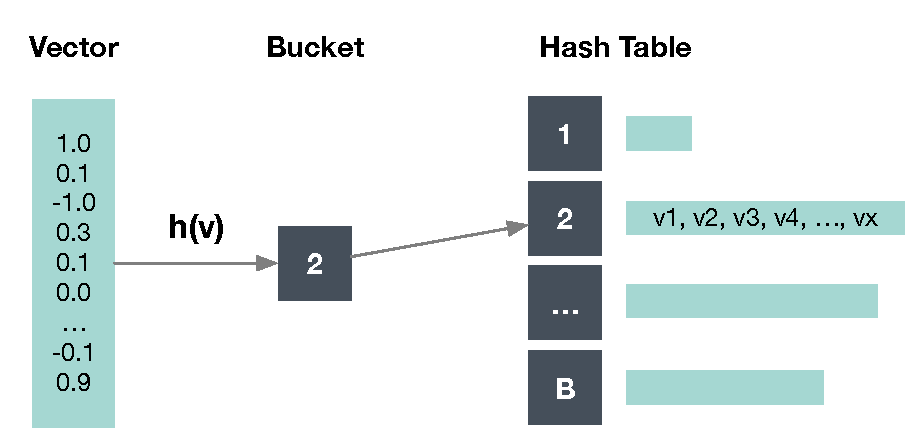
\includegraphics[width=0.75\textwidth]{figures/lsh}
    \caption{A simplified illustration of the basic \acrshort{lsh} indexing scheme. A vector is hashed to a bucket by a locality preserving hash function $h$ and stored in a hash table.}
    \label{fig:lsh}
\end{figure}

Speed-up for \acrshort{nns} can be achieved by limiting distance calculation to the vectors in the bucket a query $q$ falls into. This is referred to as non-exhaustive search. However, due to the probabilistic nature of the hash function, this type of search strategy may exhibit errors due to vectors that were hashed into the ``wrong'' bucket. More refined strategies can be employed, including hash-code ranking as well as single- and multi-table lookup \cite{Wang:2017ASurvey} to further minimise that error. Nevertheless, \acrshort{lsh} remains an approximate search strategy. A survey of different LSH algorithms can be found in \cite{Wang:2017ASurvey}.

\subsubsection{\texorpdfstring{\acrfull{pq}}{Product Quantisation (PQ)}}
\label{section:index_pq}

The idea for \acrshort{pq} was proposed by \cite{Jegou:2010Product} and it describes a technique for quantising high-dimensional vectors. The main idea involves decomposition of the original vector space $\symreal^d$ into smaller subspaces $\symreal^s$ with $s < d$ and separate quantisation of each subspace. The quantisation is achieved by learning a codebook for every subspace through k-means clustering on a representative sample of the data. Upon indexing, all subvectors of each feature vector $f \in \symfeatures$ are assigned to the nearest centroid in the codebook for the respective subspace. Concatenation of the centroid indexes gives rise to a compact signature that can be stored in an index, as illustrated in \Cref{fig:pq}.

\begin{figure}[tb]
    \centering
    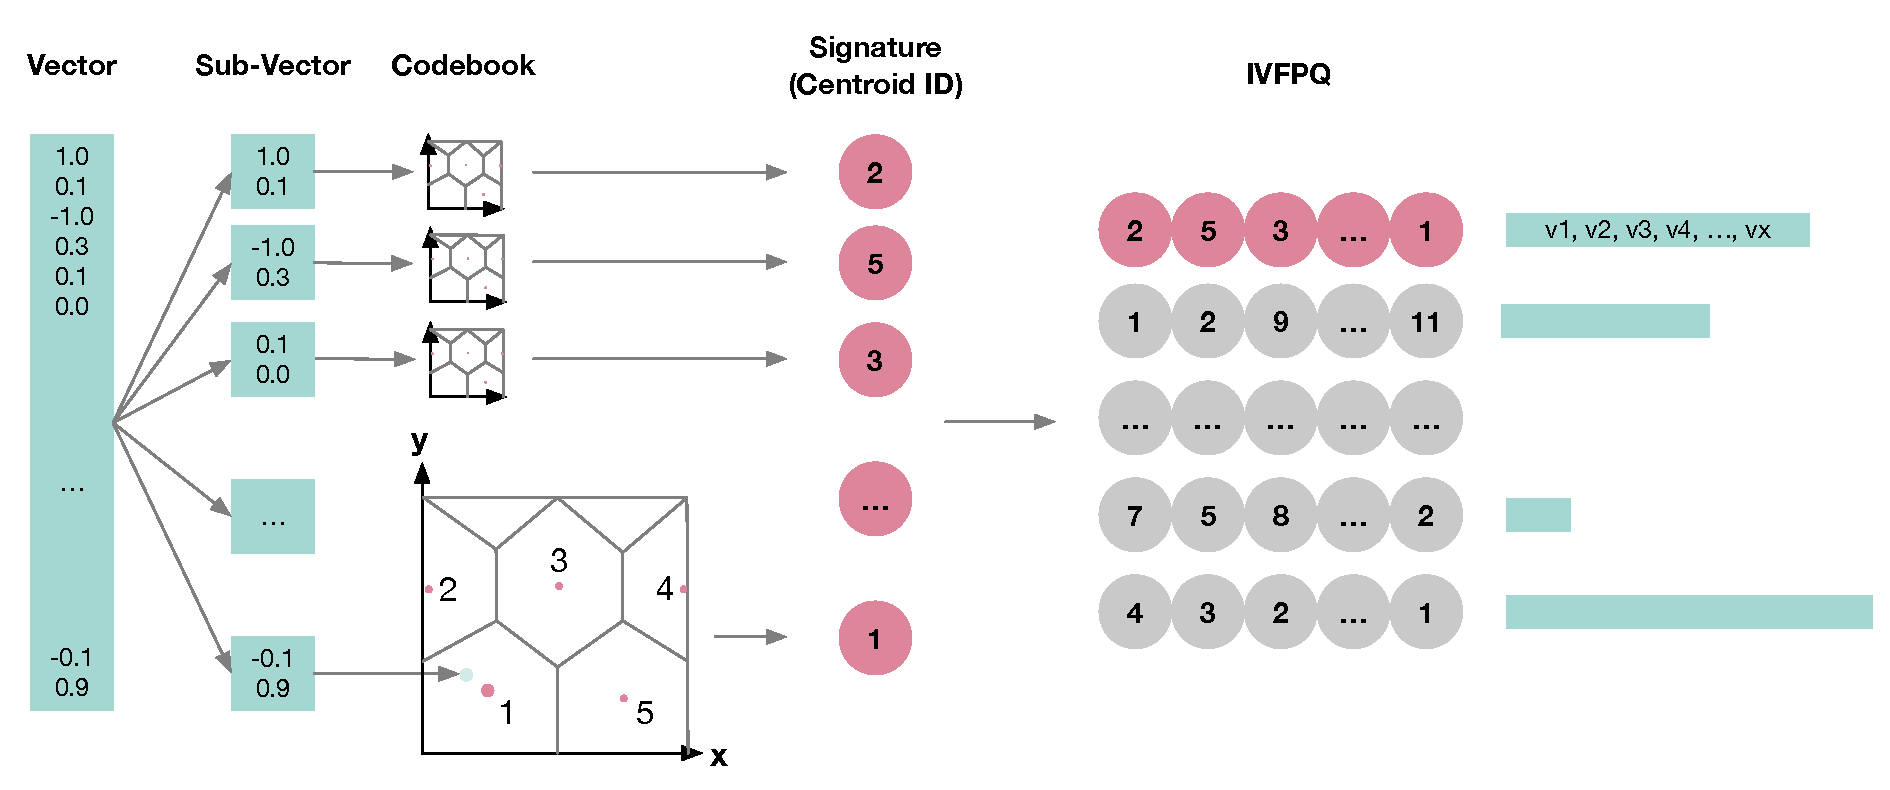
\includegraphics[width=0.95\textwidth]{figures/pq}
    \caption{A simplified illustration of the basic \acrshort{pq} indexing scheme. A vector is divided into smaller subvectors and each subvector is assigned to the nearest centroid in the codebook of the respective subspace, which produces the signature.}
    \label{fig:pq}
\end{figure}

Speed-up of \acrshort{nns} is achieved in two ways: Firstly, the resulting signature is a highly compressed representation of the original vector, which reduces \acrshort{io} by a large margin as is demonstrated in \Cref{example:pq_compression}. Secondly, the signature can be used to approximate the distance between a query $q$ and a feature $f$ using a pre-calculated lookup table and inexpensive operations, which significantly reduces CPU costs. However, this speed-up is bought by a distortion of the approximated distance, which may lead to errors if features lie very close to one another and makes PQ a suboptimal fit if exact distance values are required. \cite{Jegou:2010Product} also discusses several optimisations, e.g., encoding the difference between feature vector and centroid -- the residual -- and to use an additional, coarse quantiser to assign vectors to entries in an inverted file index (IVFPQ).

\begin{example}[label=example:pq_compression]{Size of PQ-Signature vs. original feature}{}
    Let us assume $\symfeatures \subset \symreal^{256}$, i.e., a $256$-dimensional vector space ($d = 256$). Assuming a \texttt{float} data type, we require \SI{4}{\byte} per vector component, i.e., \SI{1024}{\byte} to store a single vector.
    
    Using \acrshort{pq}, this space could now be divided into $16$ subspaces with a dimensionality of $16$ each, i.e., $s = 16 < d$. If now we assume, that we create a codebook consisting of $128$ clusters for each subspace, then every subvector will be assigned to one of $128$ centroids, which will result in $16$ numbers (one per subspace) between $0$ and $127$. Each of these numbers can be stored in a single \texttt{byte}, meaning, we only need \SI{16}{\byte} per vector to store an index entry.
\end{example}

\subsection{Beyond Similarity Search}
As we have argued in \Cref{section:application_retrieval}, the query workloads in real-world multimedia retrieval systems are often far more diverse than what we have described so far. In addition to one-shot queries, users find themselves searching, refining, browsing and exploring datasets with the aim of finding a particular item or a class of items \cite{Lokovc:2019Interactive,Rossetto:2020Interactive}. This is exemplified by interactive retrieval competitions such as \acrshort{vbs} \cite{Schoeffmann:2019Video,Lokovc:2018Influential} or \acrshort{lsc} \cite{Gurrin:2021Introduction}, where participants are required to find items of interest in large, standardised data collections \cite{Berns:2019V3C1,Rossetto:2021Insights} within a limited amount of time.

The many participants to the aforementioned campaigns have demonstrated interesting techniques that complement or even replace mere similarity search. While the 2022 instalment of \acrshort{vbs} was won by a system combining search using the CLIP model \cite{Radford:2021Learning} and sophisticated browsing \cite{Hezel:2022Efficient}, the team behind \cite{Kratochvil:2020SOM} has won the 2020 iteration of \acrshort{vbs} with a system that relies on \glsentryfirstplural{som} \cite{Kohonen:1990Self} to generate clustered visualisations of the high-dimensional data collection initialised by search input. Similarly, the system that won in 2016 \cite{Barthel:2016Navigating} used hierarchical graphs and visually sorted image maps to facilitate exploration without providing any classical search functionality. Generally, it was found that efficient browsing and exploration is as important for effective retrieval as an effective similarity search model \cite{Lokovc:2019Interactive}. A similar comparison of systems at the \acrshort{lsc} 2018 has shown, that a combination of functionality that complements similarity search is very common, including functions such as Boolean search on biometric data, facet filters, and visual clustering \cite{Gurrin:2019Invited}. Hence, as argued before, multimedia retrieval goes way beyond mere similarity search but often relies on it to some extent.

The trend away from mere search seems to have gained traction over the past few years: The Exquisitor system \cite{Ragnarsdottir:2019Exquisitor}, for example, which participated to both \acrshort{lsc} \cite{Khan:2021Exquisitor} and \acrshort{vbs} \cite{Khan:2022Exquisitor}, mainly uses relevance-feedback to train and adapt a semantic classifier (interactive learning). The ViRMA system \cite{Duane:2022ViRMA}, also present at both \acrshort{lsc} and \acrshort{vbs}, provides sophisticated, multi-dimensional exploration in virtual reality which is enabled by the $M^3$ data model \cite{Duane:2021ViRMA}. That very same model was also used by the PhotoCube system \cite{Shin2021:Photocube}, however, using a traditional desktop UI. Nevertheless, to some extent that transition also seems to be fueled by the novel means of interaction offered by virtual reality and 3D visualisation \cite{Spiess:2021Competitive,Spiess:2021Exploring,Spiess:2022Multi}.